\documentclass[journal,12pt,twocolumn]{IEEEtran}
\usepackage{setspace}
\usepackage{gensymb}
\usepackage{xcolor}
\usepackage{caption}
\singlespacing
\usepackage{siunitx}
\usepackage[cmex10]{amsmath}
\usepackage{mathtools}
\usepackage{hyperref}
\usepackage{amsthm}
\usepackage{mathrsfs}
\usepackage{txfonts}
\usepackage{stfloats}
\usepackage{cite}
\usepackage{cases}
\usepackage{subfig}
\usepackage{longtable}
\usepackage{multirow}
\usepackage{enumitem}
\usepackage{mathtools}
\usepackage{listings}
\usepackage{tikz}
\usetikzlibrary{shapes,arrows,positioning}
\usepackage{circuitikz}
\let\vec\mathbf
\DeclareMathOperator*{\Res}{Res}
\renewcommand\thesection{\arabic{section}}
\renewcommand\thesubsection{\thesection.\arabic{subsection}}
\renewcommand\thesubsubsection{\thesubsection.\arabic{subsubsection}}

\renewcommand\thesectiondis{\arabic{section}}
\renewcommand\thesubsectiondis{\thesectiondis.\arabic{subsection}}
\renewcommand\thesubsubsectiondis{\thesubsectiondis.\arabic{subsubsection}}
\hyphenation{op-tical net-works semi-conduc-tor}

\lstset{
	language=Python,
	frame=single, 
	breaklines=true,
	columns=fullflexible
}
\begin{document}
	\theoremstyle{definition}
	\newtheorem{theorem}{Theorem}[section]
	\newtheorem{problem}{Problem}
	\newtheorem{proposition}{Proposition}[section]
	\newtheorem{lemma}{Lemma}[section]
	\newtheorem{corollary}[theorem]{Corollary}
	\newtheorem{example}{Example}[section]
	\newtheorem{definition}{Definition}[section]
	\newcommand{\BEQA}{\begin{eqnarray}}
		\newcommand{\EEQA}{\end{eqnarray}}
	\newcommand{\define}{\stackrel{\triangle}{=}}
	\newcommand{\myvec}[1]{\ensuremath{\begin{pmatrix}#1\end{pmatrix}}}
	\newcommand{\mydet}[1]{\ensuremath{\begin{vmatrix}#1\end{vmatrix}}}
	\bibliographystyle{IEEEtran}
	\providecommand{\nCr}[2]{\,^{#1}C_{#2}} % nCr
	\providecommand{\nPr}[2]{\,^{#1}P_{#2}} % nPr
	\providecommand{\mbf}{\mathbf}
	\providecommand{\pr}[1]{\ensuremath{\Pr\left(#1\right)}}
	\providecommand{\qfunc}[1]{\ensuremath{Q\left(#1\right)}}
	\providecommand{\sbrak}[1]{\ensuremath{{}\left[#1\right]}}
	\providecommand{\lsbrak}[1]{\ensuremath{{}\left[#1\right.}}
	\providecommand{\rsbrak}[1]{\ensuremath{{}\left.#1\right]}}
	\providecommand{\brak}[1]{\ensuremath{\left(#1\right)}}
	\providecommand{\lbrak}[1]{\ensuremath{\left(#1\right.}}
	\providecommand{\rbrak}[1]{\ensuremath{\left.#1\right)}}
	\providecommand{\cbrak}[1]{\ensuremath{\left\{#1\right\}}}
	\providecommand{\lcbrak}[1]{\ensuremath{\left\{#1\right.}}
	\providecommand{\rcbrak}[1]{\ensuremath{\left.#1\right\}}}
	\theoremstyle{remark}
	\newtheorem{rem}{Remark}
	\newcommand{\sgn}{\mathop{\mathrm{sgn}}}
	\newcommand{\rect}{\mathop{\mathrm{rect}}}
	\newcommand{\sinc}{\mathop{\mathrm{sinc}}}
	\providecommand{\abs}[1]{\left\vert#1\right\vert}
	\providecommand{\res}[1]{\Res\displaylimits_{#1}} 
	\providecommand{\norm}[1]{\lVert#1\rVert}
	\providecommand{\mtx}[1]{\mathbf{#1}}
	\providecommand{\mean}[1]{E\left[ #1 \right]}
	\providecommand{\fourier}{\overset{\mathcal{F}}{ \rightleftharpoons}}
	\providecommand{\ztrans}{\overset{\mathcal{Z}}{ \rightleftharpoons}}
	\providecommand{\system}[1]{\overset{\mathcal{#1}}{ \longleftrightarrow}}
	\newcommand{\solution}{\noindent \textbf{Solution: }}
	\providecommand{\dec}[2]{\ensuremath{\overset{#1}{\underset{#2}{\gtrless}}}}
	\numberwithin{equation}{section}
	\makeatletter
	\@addtoreset{figure}{problem}
	\makeatother
	\let\StandardTheFigure\thefigure
	\renewcommand{\thefigure}{\theproblem}
	\def\putbox#1#2#3{\makebox[0in][l]{\makebox[#1][l]{}\raisebox{\baselineskip}[0in][0in]{\raisebox{#2}[0in][0in]{#3}}}}
	\def\rightbox#1{\makebox[0in][r]{#1}}
	\def\centbox#1{\makebox[0in]{#1}}
	\def\topbox#1{\raisebox{-\baselineskip}[0in][0in]{#1}}
	\def\midbox#1{\raisebox{-0.5\baselineskip}[0in][0in]{#1}}
   
\title{ Digital Signal Processing \\ \Large EE3900 \\ \vspace*{12pt} \textbf{Fourier Series}}
\author{I Sai Pradeep\\ \normalsize AI21BTECH11013 \\ \vspace*{20pt} \normalsize \today}
 \maketitle 
 \tableofcontents
 \begin{abstract}
    This manual provides a simple introduction to Fourier Series
    \end{abstract}
    \section{Periodic Function}
    Let 
    \begin{align}
        x(t) &= A_0\abs{\sin\brak{2\pi f_0 t}}
        \label{eq:x(t)}
    \end{align}
    \begin{enumerate}[label=\thesection.\arabic*
    ,ref=\thesection.\theenumi]
    \item Plot $x(t)$.\\
    \solution 
    \begin{lstlisting}
wget https://github.com/Pradeep8802/EE3900-Digital-Signal-Processing/blob/main/charger/codes/1.1.py
    \end{lstlisting}
    \begin{figure}[!ht]
			\centering
			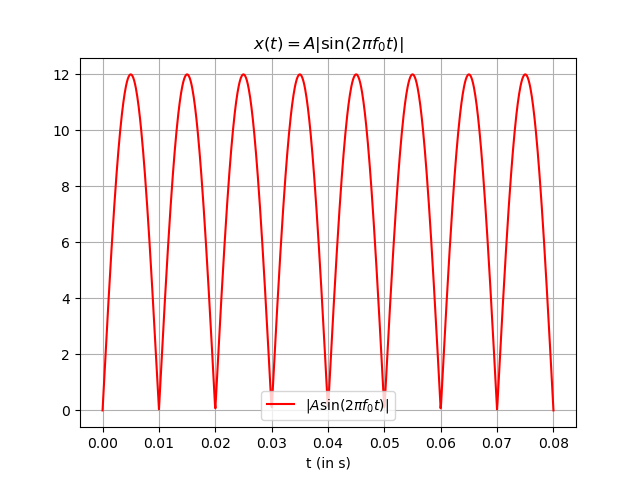
\includegraphics[width=\columnwidth]{./figs/1.1.png}
			\caption{}
			%\label{fig:ckt}
\end{figure}
    \item Show that $x(t)$ is periodic and find its period.
    \solution 
    A signal $x(t)$ is said to be periodic with fundamental period $T$ if
    \begin{align}
    \label{eq:peroidic}
    x(t+nT)=x(t) \forall n \in \mathbb{Z}
    \end{align}
Let $T$ be fundamental period of $x(t)$. Comparing \eqref{eq:peroidic} and \eqref{eq:x(t)}, we get
	\begin{align}
A_0\abs{\sin\brak{2\pi f_0 t}}&=A_0\abs{\sin\brak{2\pi f_0 (t+T)}}\\
\abs{\sin\brak{2\pi f_0 t}}&=\abs{\sin\brak{2\pi f_0 (t+T)}}\\
\abs{\sin\brak{2\pi f_0 t}}&=\abs{\sin\brak{2\pi f_0 t+2\pi f_0 T)}}
	\end{align}
As $|sin\theta|$ is periodic with fundamental period $F=\pi$, Hence,
    \begin{align}
\abs{\sin\brak{t}}=\abs{\sin\brak{t+F)}}
\end{align}
Hence,$2\pi f_0  T=\pi$, therefore, fundamental period($T$) is 
\begin{align}
\label{eq:ftp}
T=\frac{\pi}{2 \pi f_0}=\frac{1}{2f_0}
    \end{align}
    \end{enumerate}
    \section{Fourier Series}
    Consider $A_0 =12$ and $f_0 = 50$ for all numerical calculations.
    \begin{enumerate}[label=\thesection.\arabic*,ref=\thesection.\theenumi]
    \item If
    %\cite{proakis_dsp}
    \begin{align}
        x(t) = \sum_{k = -\infty}^{\infty}c_ke^{j2\pi kf_0 t}
    \label{eq:one-Z-complex}
    \end{align}
    show that 
    \begin{align}
        c_k = f_0\int_{-\frac{1}{2f_0}}^{\frac{1}{2f_0}}x(t)e^{-j2\pi kf_0 t}\, dt
    \label{eq:one-Z}
    \end{align}
    \solution 
    From \eqref{eq:one-Z-complex},
    \begin{align}
    	\label{eq:sum}
            x(t) = \sum_{k = -\infty}^{\infty}c_ke^{j2\pi kf_0 t}
    \end{align}
    Mulitply $e^{-j2\pi lf_0 t}$ on both sides of \eqref{eq:sum}, we get,
    \begin{align}
    	\label{eq:a}
    x(t)e^{-j2\pi lf_0 t}=\sum_{k = -\infty}^{\infty}c_ke^{j2\pi kf_0 t}e^{-j2\pi lf_0 t}
    \end{align}
    Integrating \eqref{eq:a} w.r.t. $t$ from $-T$ to $T$, and $T=\frac{1}{f_0}$, we get,\\
    \begin{align}
    	\label{eq:d}
    \int_{-\frac{1}{2f_0}}^{\frac{1}{2f_0}}x(t)e^{-j2\pi kf_0 t}\, dt&=\int_{-\frac{1}{2f_0}}^{\frac{1}{2f_0}}\sum_{k = -\infty}^{\infty}c_ke^{j2\pi \brak{k-l}f_0 t}\,dt\\
    &=\sum_{k = -\infty}^{\infty}c_k\int_{-\frac{1}{2f_0}}^{\frac{1}{2f_0}}e^{j2\pi \brak{k-l}f_0 t}\,dt
    \end{align}
Consider the following cases.\\
case-1:$k=l$
\begin{align}
	\int_{-\frac{1}{2f_0}}^{\frac{1}{2f_0}}e^{j2\pi \brak{k-l}f_0 t}\,dt&=\int_{-\frac{1}{2f_0}}^{\frac{1}{2f_0}}e^{0}\,dt\\
	&=\int_{-\frac{1}{2f_0}}^{\frac{1}{2f_0}} 1 \,dt
\end{align}
case-2: $k \neq l$ \\
Let $n=f_0(k-l)$, here $n \in \mathbb{Z}$
\begin{align}
	\label{eq:b}
\int_{-\frac{1}{2f_0}}^{\frac{1}{2f_0}}e^{j2\pi \brak{k-l}f_0 t}\,dt&=\int_{-\frac{1}{2f_0}}^{\frac{1}{2f_0}}e^{2n\pi}\,dt	
\end{align}
Here, $2n\pi T=2f_0(k-l)T\pi$, and $2n\pi T=(k-l)\pi$
\begin{align}
\int_{-\frac{1}{2f_0}}^{\frac{1}{2f_0}}e^{j2n\pi}\,dt&=\int_{-\frac{1}{2f_0}}^{\frac{1}{2f_0}}1\,dt\\&=\int_{-\frac{1}{2f_0}}^{\frac{1}{2f_0}}\cos(2n\pi)+j\sin(2n\pi) \,dt
\end{align}
\begin{align}
\int_{-\frac{1}{2f_0}}^{\frac{1}{2f_0}}e^{j2n\pi}\,dt&=
-\sin(2n\pi t)\bigg|_{-\frac{1}{2f_0}}^{\frac{1}{2f_0}}\\&+j\cos(2n\pi t)\bigg|_{-\frac{1}{2f_0}}^{\frac{1}{2f_0}}\\
&=-\sin(2n\pi t)\bigg|_{-\frac{1}{2f_0}}^{\frac{1}{2f_0}}\\&+j\cos(2n\pi t)\bigg|_{-\frac{1}{2f_0}}^{\frac{1}{2f_0}}\\
&=-\sin(2n\pi t)\bigg|_{-\frac{1}{2f_0}}^{\frac{1}{2f_0}}\\&+j\cos(2n\pi t)\bigg|_{-\frac{1}{2f_0}}^{\frac{1}{2f_0}}\\
\label{eq:c}\\
&=-\sin((k-l)\pi)+\sin(-(k-l)\pi)\\&+j\cos((k-l)\pi)-j\cos(-(k-l)\pi)\\
\end{align}
Since $k-l \in \mathbb{Z}$,$\sin((k-l)\pi)=0$ and $\sin(-(k-l)\pi)=0$, simillarly, as $\cos(\theta)=\cos(-\theta)$, we get $\cos((k-l)\pi)-\cos(-(k-l)\pi)=0$\\
From \eqref{eq:c},
\begin{align}
	\int_{-\frac{1}{2f_0}}^{\frac{1}{2f_0}}e^{j2n\pi}\,dt&=\int_{-\frac{1}{2f_0}}^{\frac{1}{2f_0}}1\,dt\\&=0+j0=0
\end{align}
Hence, we have,
    \begin{align}
\int_{-\frac{1}{2f_0}}^{\frac{1}{2f_0}}e^{j2\pi \brak{k-l}f_0 t}\,dt=
         \begin{cases}
0 & k\neq l
\\
 \int_{-\frac{1}{2f_0}}^{\frac{1}{2f_0}}1\,dt& k=l
\end{cases}
    \end{align}
From \eqref{eq:d},
    \begin{align}
    	\int_{-\frac{1}{2f_0}}^{\frac{1}{2f_0}}x(t)e^{-j2\pi kf_0 t}\, dt&=\sum_{k = -\infty}^{\infty}c_k\int_{-\frac{1}{2f_0}}^{\frac{1}{2f_0}}e^{j2\pi \brak{k-l}f_0 t}\,dt\\
    	&=c_k \times \int_{-\frac{1}{2f_0}}^{\frac{1}{2f_0}}1\,dt
    	\end{align}
    \begin{align}
  c_k &= f_0\int_{-\frac{1}{2f_0}}^{\frac{1}{2f_0}}x(t)e^{-j2\pi kf_0 t}\, dt\\
  \therefore c_k &= \frac{2}{T} \int_{-\frac{1}{T}}^{\frac{1}{T}}x(t)e^{-j2\pi kf_0 t}\, dt
    \end{align}
        \item Find $c_k$ for 
        \eqref{eq:x(t)}\\
        \solution
        We know that,
        \begin{align}
        c_k = 2f_0\int_{0}^{\frac{1}{2f_0}}x(t)e^{- j2 \pi kf_0 t}\, dt
        \end{align}
when $t \in \bigg( 0,\frac{1}{2f_0}\bigg)$, $x(t)=A_0 \sin\brak{2 \pi f_0t}$\\
      \begin{align}
      c_k &= 2f_0\int_{0}^{\frac{1}{2f_0}}A_0 \brak{\frac{e^{j2\pi f_0t}-e^{-j 2\pi f_0t}}{2j}} e^{- j2 \pi kf_0 t}\,dt\\
      &=A_0f_0\int_{0}^{\frac{1}{2f_0}} \brak{\frac{e^{j2\pi\brak{1-k} f_0t}-e^{j 2\pi\brak{-1-k} f_0t}}{j}}\,dt\\
&=A_0f_0\bigg(\frac{e^{j2\pi\brak{1-k} f_0t}}{-2\pi \brak{1-k}f_0}\bigg|_0^{\frac{1}{2f_0}} \\&- \frac{e^{j2\pi\brak{-1-k} f_0t}}{-2\pi \brak{-1-k}f_0}\bigg|_0^{\frac{1}{2f_0}}\bigg)\\
&=A_0\sbrak{\frac{e^{j\pi\brak{1-k}}-1}{2\pi\brak{k-1}}-\frac{e^{-j\pi\brak{1+k}}-1}{2\pi\brak{k+1}}}
      \end{align}
  Hence,
      \begin{equation}
      \label{eq:ck}
     c_k= \begin{cases}
\frac{2A_0}{\pi\brak{1-k^2}}&k=even
\\
0&k=odd
\end{cases}
      \end{equation}
    \item Verify 
        \eqref{eq:x(t)}
        using python.\\
        \solution 
        \begin{lstlisting}
wget https://github.com/Pradeep8802/EE3900-Digital-Signal-Processing/blob/main/charger/codes/2.3.py
        python3 2.3.py
        \end{lstlisting}
          \begin{figure}[!ht]
			\centering
			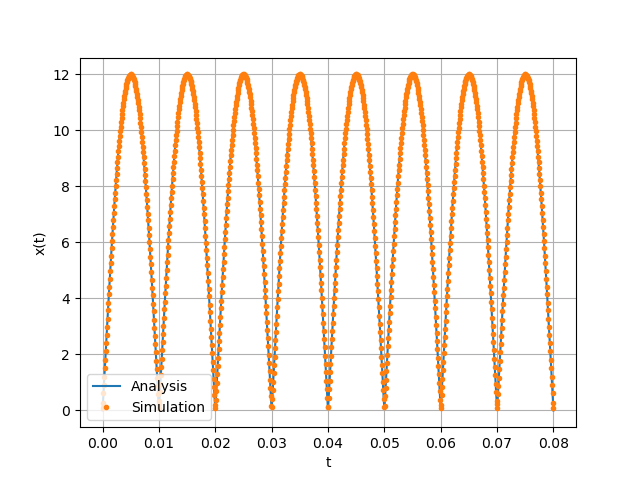
\includegraphics[width=\columnwidth]{./figs/2.3.png}
			\caption{}
			%\label{fig:ckt}
\end{figure}
         \item Show that 
    \begin{align}
        x(t) = \sum_{k = 0}^{\infty}\brak{a_k\cos{2\pi kf_0 t}+b_k\sin{2\pi kf_0 t}}
    \label{eq:one-Z-real}
    \end{align}
    and obtain the formulae for $a_k$ and $b_k$.\\
    \solution
    Using \eqref{eq:one-Z-complex},
    \begin{align}
    x(t) = \sum_{k = -\infty}^{\infty}c_ke^{j2\pi kf_0 t}
    \end{align}
    As,
    \begin{align}
    e^{j2\pi kf_0 t}=\cos\brak{2\pi kf_0 t}+j\sin\brak{2\pi kf_0 t}
    \end{align}
    From \eqref{eq:one-Z-complex}, we have,
    \begin{align}
    x(t) &= \sum_{k = -\infty}^{\infty}c_k\sbrak{\cos\brak{2\pi kf_0 t}+j\sin\brak{2\pi kf_0 t}}\\
    \label{eq:2.4}
    &=\sum_{k = -\infty}^{\infty}c_k\cos\brak{2\pi kf_0 t}+jc_k\sin\brak{2\pi kf_0 t}\\
    &=\sum_{k = -\infty}^{-1}\sbrak{c_k\cos\brak{2\pi kf_0 t}+jc_k\sin\brak{2\pi kf_0 t}} \\ &+c_0+\sum_{k = 1}^{\infty}\sbrak{c_k\cos\brak{2\pi kf_0 t}+jc_k\sin\brak{2\pi kf_0 t}}\\
    &=\sum_{k = 1}^{\infty}\sbrak{c_{-k}\cos\brak{2\pi kf_0 t}-jc_{-k}\sin\brak{2\pi kf_0 t}}\\ &+c_0+\sum_{k = 1}^{\infty}\sbrak{c_k\cos\brak{2\pi kf_0 t}+jc_k\sin\brak{2\pi kf_0 t}}\\
    &=c_0+\sum_{k = 1}^{\infty}\bigg(\brak{c_k+c_{-k}}\cos\brak{2\pi kf_0 t}\\ &+j\brak{c_k-c_{-k}}\sin\brak{2\pi kf_0 t}\bigg)
    \end{align}
    Substituting $a_k=c_{k} + c_{-k}$ and $b_k=j(c_{k}-c_{-k})$,we get,
    \begin{align}
x(t)&=c_0+    \sum_{k = 1}^{\infty}\brak{a_k\cos{2\pi kf_0 t}+b_k\sin{2\pi kf_0 t}}\\
&=\sum_{k = 0}^{\infty}\brak{a_k\cos{2\pi kf_0 t}+b_k\sin{2\pi kf_0 t}}
    \end{align}
    \begin{align}
    \label{eq:u1}
    \therefore a_k&=
    \begin{cases}
    c_k+c_{-k}&k\neq0
    \\
    c_0&k=0
    \end{cases}\\
    \label{eq:u2}
    b_k&=j\brak{c_k-c_{-k}}
    \end{align}
    Using \eqref{eq:one-Z},
    \begin{align}
    c_k &= f_0\int_{-\frac{1}{2f_0}}^{\frac{1}{2f_0}}x(t)e^{-j2\pi kf_0 t}\, dt\\
    c_{-k} &= f_0\int_{-\frac{1}{2f_0}}^{\frac{1}{2f_0}}x(t)e^{j2\pi kf_0 t}\, dt\end{align}
    \begin{align}
    a_k=c_k+c_{-k}&= f_0\int_{-\frac{1}{2f_0}}^{\frac{1}{2f_0}}x(t)\sbrak{e^{-j2\pi kf_0 t}+e^{j2\pi kf_0 t}}\, dt\\
    &=2f_0\int_{-\frac{1}{2f_0}}^{\frac{1}{2f_0}}x(t)\cos\brak{2\pi kf_0t}\, dt
    \end{align}
    Similarly, for $b_k$, we get,
    \begin{align}
    b_k=-j\cbrak{2f_0\int_{-\frac{1}{2f_0}}^{\frac{1}{2f_0}}x(t)\sin\cbrak{2\pi kf_0t}\, dt}
    \end{align}
    \item Find $a_k$ and $b_k$ for 
        \eqref{eq:x(t)}\\
        \solution
        Using \eqref{eq:u1} and \eqref{eq:u2} with \eqref{eq:ck},
    \begin{align}
    a_k&=c_k+c_{-k}=\begin{cases}
\frac{4A_0}{\pi\brak{1-k^2}}&k=even
\\
\frac{2A_0}{\pi}&k=0
\\
0&k=odd
\end{cases}\\
b_k&=j\brak{c_k-c_{-k}}=0
    \end{align}
    \item Verify 
    \eqref{eq:one-Z-real}
    using python.\\
     \solution 
        \begin{lstlisting}
wget https://github.com/Pradeep8802/EE3900-Digital-Signal-Processing/blob/main/charger/codes/2.6.py
        python3 2.3.py
        \end{lstlisting}
          \begin{figure}[!ht]
			\centering
			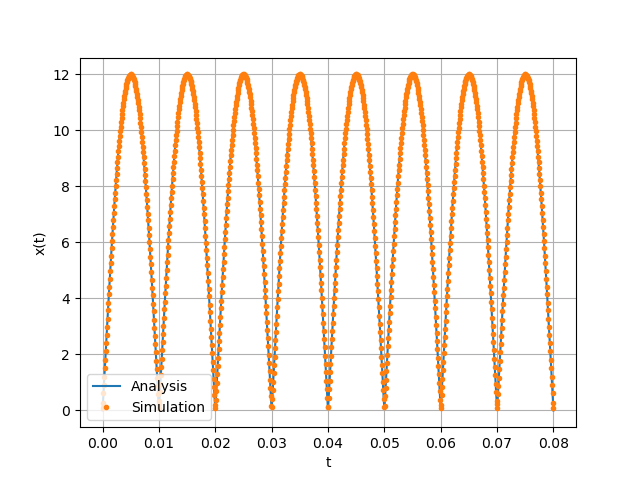
\includegraphics[width=\columnwidth]{./figs/2.6.png}
			\caption{}
			%\label{fig:ckt}
\end{figure}
    \end{enumerate}
\section{Fourier Transform}
\begin{enumerate}[label=\thesection.\arabic*
	,ref=\thesection.\theenumi]
	\item 
	\begin{align}
		\delta(t)&=0, \quad t\neq 0 \\
		\int_{-\infty}^{\infty}\delta(t) \, dt&= 1
	\end{align}
	\item The Fourier Transform of $g(t)$ is
	\begin{align}
		G(f)=\int_{-\infty}^{\infty}g(t)e^{-j2\pi ft}\,dt
		\label{eq:fourier}
	\end{align}
	\item Show that 
	\begin{align}
		g(t-t_0)&\system{F}G(f)e^{-j2\pi ft_0}
		\label{eq:t-shift}
	\end{align}
	\solution Let us consider $x=t-t_0$. Fourier transform of $g(t-t_0)$ is given as
	\begin{align}
		g(t-t_0)&\system{F}\int_{-\infty}^{\infty}
		g(t-t_0)e^{-\j2\pi ft}\,dt \\
		&=\int_{-\infty}^{\infty}
		g(t-t_0)e^{-\j2\pi f((t-t_0) + t_0)}\,du \\
		&=\int_{-\infty}^{\infty}
		g(x)e^{-j2\pi f(x+t_0)}\,dt\\
		&=\int_{-\infty}^{\infty}
		g(x)e^{-j2\pi f(x+t_0)}\,d(x-t_0)\\
		&=\int_{-\infty}^{\infty}
		e^{-\j2\pi f t_0}g(x)e^{-j2\pi fx}\,d(x)\\
		\label{eq:3.3}
		&=e^{-\j2\pi f t_0} \cbrak{\int_{-\infty}^{\infty}
		g(x)e^{-\j2\pi fx}\,d(x)}
	\end{align}
Using \eqref{eq:fourier} in equation \eqref{eq:3.3}, we get,
\begin{align}
	\label{eq:3.3.1}
	g(t-t_0)\system{F}G(f)e^{-\j2\pi ft_0}
	\end{align}
	\item Show that
	\begin{align}
		\label{eq:inverse}
		G(t)&\system{F}g(-f)
	\end{align}
	\solution 
	Let $g(t)\system{F}G(f)$ , then 
	\begin{align}
		\label{eq:inverseFourier}
		g(t)=\int_{-\infty}^{\infty}G(f)e^{\j2\pi ft}\,df
	\end{align}
Consider $g(-k)$,
\begin{align}
	g(-k)=\int_{-\infty}^{\infty}G(f)e^{\j2\pi fk}\,df
\end{align}
Let $f=t$,then,
\begin{align}
	\label{eq:3.4}
	g(-k)=\int_{-\infty}^{\infty}G(t)e^{\j2\pi tk}\,dt
\end{align}
Substituting $k=f$ and in the \eqref{eq:3.4}, we get, 
\begin{align}
	\label{eq:3.4.1}
	g(-f)=\int_{-\infty}^{\infty}G(t)e^{\j2\pi ft}\,dt
\end{align}
Comparing \eqref{eq:3.4.1} with \eqref{eq:fourier}, we can say that,
\begin{align}
	G(t)&\system{F}g(-f)
\end{align}
%	\begin{align}
%		g(t)=\int_{-\infty}^{\infty}G(f)e^{\j2\pi ft}\,df
%		\label{eq:duality}
%	\end{align}
%	Hence, setting $t := -f$ and $f := t$, which implies $df = dt$,
%	\begin{align}
%		g(-f)&=\int_{-\infty}^{\infty}G(t)e^{-\j2\pi ft}\,dt \\
%		\implies G(t)&\system{F}g(-f)
%	\end{align}
	\item $\delta(t)\system{F}?$\\
	\solution From \eqref{eq:fourier}, fourier transform of $\delta(t)$ is,
	\begin{align}
		\delta(t)&\system{F} \int_{-\infty}^{\infty}\delta(t) e^{-\j2\pi ft} \,dt\\
		&=\int_{-\infty}^{\infty}\delta(0) e^{-\j2\pi f 0} \,dt\\
		&=\int_{-\infty}^{\infty}\delta(0) \,dt \\
		&=1
	\end{align}
Hence,
$\delta(t) \system{F} 1$
%	We have, from the definition of $\delta(t)$,
%	\begin{align}
%		\delta(t)&\system{F}\int_{-\infty}^{\infty}\delta(t)e^{-\j2\pi ft}\, dt \\
%		&=\int_{-\infty}^{\infty}\delta(0)\, dt \\
%		&=\int_{-\infty}^{\infty}\delta(t)\, dt = 1
%		\label{eq:fourier-delta}
%	\end{align}
	\item $e^{-j2\pi f_0t}\system{F}?$\\
	\solution Suppose $g(t)\system{F}G(f)$. Hence,
\begin{align}
	g(t)&\system{F} \int_{-\infty}^{\infty}g(t)e^{-\j2\pi ft}\\
	g(t)e^{-j2\pi f_0t}&\system{F} \int_{-\infty}^{\infty}g(t)e^{-\j2\pi ft}e^{-j2\pi f_0t}\\
	g(t)e^{-j2\pi f_0t}&\system{F} G(f)e^{-j2\pi f_0 f}\\
\end{align}
From \eqref{eq:3.4.1},
\begin{align}
	g(t-f_0)&\system{F}G(f)e^{-\j2\pi ft f_0}\\
	g(t)e^{-j2\pi f_0t}&\system{F} G(f)e^{-j2\pi f_0 f}\\
\end{align}
From \eqref{eq:inverseFourier},
\begin{align}
	\delta(t)&\system{F}1\\
	1&\system{F}\delta(-f)=\delta(f)
\end{align}
Hence, 
\begin{align}
	g(t-f_0)&\system{F} \delta((f+f_0))
\end{align}
	\begin{align}
		g(t)e^{\j2\pi f_0t}&\system{F}\int_{-\infty}^{\infty}
		g(t)e^{-\j2\pi\brak{f-f_0}t}\, dt \\
		&=G(f-f_0)
		\label{eq:f-shift}
	\end{align}
	%Using \eqref{eq:duality} in \eqref{eq:fourier-delta}, $1\system{F}\delta(-f)$.
	%Hence, applying \eqref{eq:f-shift},
	Hence,
	\begin{align}
		e^{-\j2\pi f_0t}\system{F}\delta(-(f+f_0)) = \delta(f+f_0)
		\label{eq:fourier-exp}
	\end{align}
	\item $\cos(2\pi f_0t)\system{F}?$\\
	\solution We know that 
	\begin{align}
			\cos\brak{2\pi f_0t} = \frac{1}{2}
			\brak{e^{\j2\pi f_0t} + e^{-\j2\pi f_0t}} \\
	\end{align}
Hence,
\begin{align}
\mathcal{F}(\cos\brak{2\pi f_0t})&=\mathcal{F}(\frac{1}{2}
\brak{e^{\j2\pi f_0t} + e^{-\j2\pi f_0t}})\\
\mathcal{F}(\cos\brak{2\pi f_0t})&=\frac{1}{2} \mathcal{F}(
\brak{e^{\j2\pi f_0t}})+ \frac{1}{2} \mathcal{F}(e^{-\j2\pi f_0t})\\
&=\frac{1}{2} \mathcal{F}(
\brak{e^{\j2\pi f_0t}})+ \frac{1}{2} \mathcal{F}(e^{-\j2\pi f_0t})\\
&=\frac{1}{2}\brak{\delta\brak{f-f_0} + \delta\brak{f+f_0}}
\end{align}
%
%	Using the linearity of the Fourier 
%	Transform and \eqref{fourier-exp},
%	\begin{align}
%		\cos\brak{2\pi f_0t} &= \frac{1}{2}
%		\brak{e^{\j2\pi f_0t} + e^{-\j2\pi f_0t}} \\
%		&\system{F}\frac{1}{2}\brak{\delta\brak{f+f_0} + \delta\brak{f-f_0}}
%	\end{align}
	\item Find the Fourier Transform of $x(t)$ and plot it. Verify using python.\\
	\solution As obtained earlier, from equation \eqref{eq:ck},
	\begin{align}
		x(t)=\sum_{k=-\infty}^{\infty}c_k e^{j2\pi k f_0 t}\\
		e^{j 2 \pi k f_0 t}\system{F}=\delta{f-kf_0}
	\end{align}
	Hence, from the value of $c_k$,
	\begin{align}
 x(t)&\system{F}\sum_{k=-\infty}^{\infty} \delta\brak{f+kf_0} c_k\\
		\implies x(t)&\system{F}\sum_{k=-\infty}^{\infty} \frac{2A_0}{\pi} \frac{\delta\brak{f+2kf_0}}{1-4k^2} 
	\end{align} 
	\begin{figure}[!ht]
				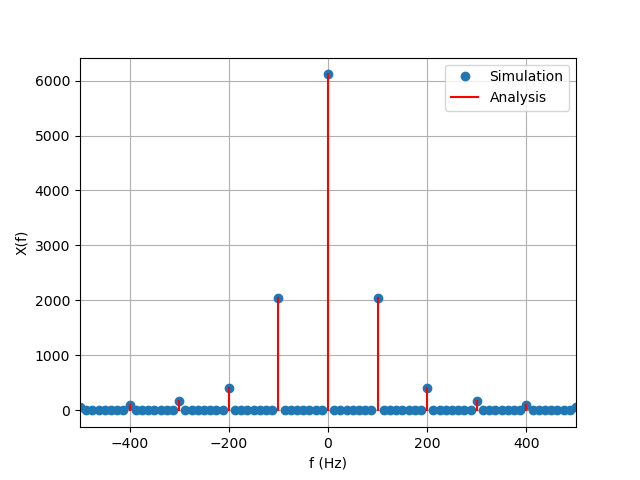
\includegraphics[width=\columnwidth]{figs/3.8.png}
				\caption{Fourier Transform of $x(t)$.}
				\label{fig:fourier-xt}
			\end{figure}
	Fourier transform of $x(t)$ is verified in the following figure. 
	The figure is plotted using the below python code.
	\begin{lstlisting}
wget https://github.com/Pradeep8802/EE3900-Digital-Signal-Processing/blob/main/charger/codes/3.8.py
	\end{lstlisting} 
%	
	\item Show that
	\begin{align}
		\rect{t} \system{F} \sinc{f}
	\end{align}
	Verify using python.\\
	\solution We know that,
	\begin{align}
		rect(t)&=
	\begin{cases}
		0 \quad t<\frac{-1}{2}\\
		1 \quad \frac{-1}{2}<t<\frac{1}{2}\\
		0 \quad t>\frac{1}{2}
	\end{cases}\\
\sinc(f)&=\frac{\sin{\pi f}}{\pi f}
	\end{align}
Applying fourier transform we get,
	\begin{align}
		\rect{t}&\system{F}\int_{-\infty}^{\infty}\rect{t} e^{-\j2\pi ft}\, dt \\
		&=\int_{-\frac{1}{2}}^{\frac{1}{2}}e^{-\j 2\pi ft}\, dt \\
		\label{eq:fourierrect}
		&=\frac{e^{\j\pi f} - e^{-\j\pi f}}{\j2\pi f} = \frac{\sin{\pi f}}{\pi f} = \sinc{f}
	\end{align}
	\begin{figure}[!ht]
	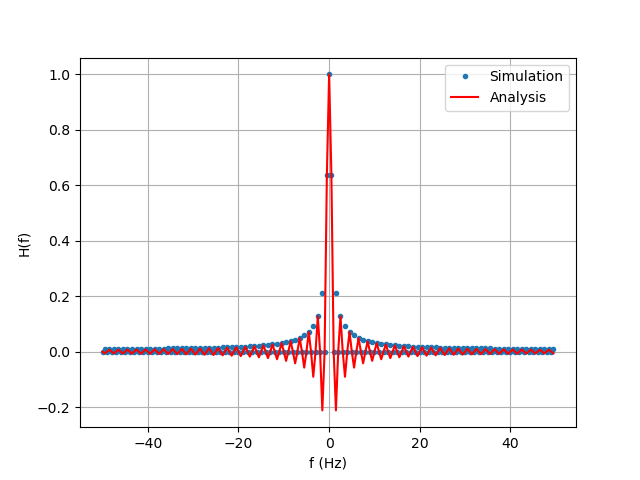
\includegraphics[width=\columnwidth]{figs/3.9.png}
	\caption{Fourier Transform of $\rect{t})$.}
	\label{fig:3.9}
\end{figure}
The below python code plots the figure \ref{fig:3.9}
	\begin{lstlisting}
	wget https://github.com/Pradeep8802/EE3900-Digital-Signal-Processing/blob/main/charger/codes/3.9.py
\end{lstlisting} 

	\item $\sinc{t}\system{F} ?$  Verify using python.\\
	\solution From \eqref{eq:3.3}, we have 
	
	\begin{align}
		\sinc{t}\system{F}\rect(-f)=\rect{f}
		\label{eq:fourier-sinc}
	\end{align}
\begin{figure}[!ht]
	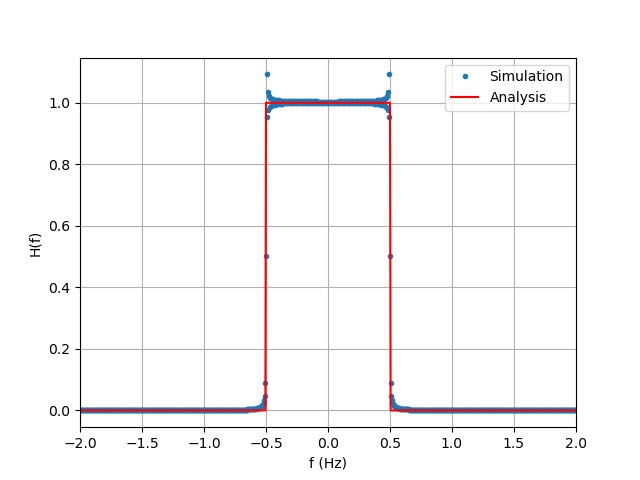
\includegraphics[width=\columnwidth]{figs/3.10.png}
	\caption{Fourier Transform of $\rect{t})$.}
	\label{fig:3.10}
\end{figure}
	Since $\rect{f}$ is an even function.
	The below python code plots the figure \ref{fig:3.10}
	\begin{lstlisting}
wget https://github.com/Pradeep8802/EE3900-Digital-Signal-Processing/blob/main/charger/codes/3.10.py
	\end{lstlisting} 

%	The python code \texttt{codes/3\_10.py} verifies \eqref{eq:fourier-sinc}
%	by plotting Fig. \ref{fig:fourier-sinc}.
%	\begin{figure}[!ht]
%		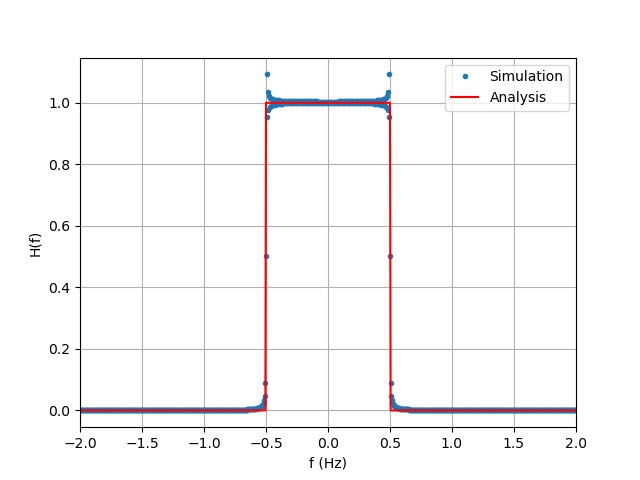
\includegraphics[width=\columnwidth]{figs/3_10.png}
%		\caption{Fourier Transform of $\sinc(t)$.}
%		\label{fig:fourier-sinc}
%	\end{figure}
\end{enumerate}
\section{Filter}
\begin{enumerate}[label=\thesection.\arabic*
	,ref=\thesection.\theenumi]
	\item Find $H(f)$ which transforms $x(t)$ to DC 5V.\\
	\solution The function $H(f)$ is a low pass filter which filters out
	even harmonics and leaves the zero frequency component behind.
	The rectangular function represents an ideal low pass filter. 
	Suppose the cutoff frequency is $f_c = 50$ Hz, then
	\begin{align}
		H(f) = \rect\brak{\frac{f}{2f_c}} =
		\begin{cases}
			1 & \abs{f} < f_c \\
			0 & \textrm{otherwise}
		\end{cases}
		\label{eq:Hfb}
	\end{align}
	Multiplying by a scaling factor to get DC 5V,
	\begin{align}
		\label{eq:Hfa}
		H(f) = \frac{\pi V_0}{2A_0}\rect{\brak{\frac{f}{2f_c}}}
	\end{align}
	where $V_0 = 5$ V.
	\item Find $h(t)$.\\
	\solution Suppose $g(t)\system{F}G(f)$. Then, for some
	nonzero $a \in \mathbb{R}$, let $u=at$,
	\begin{align}
		g(at)&\system{F}\int_{-\infty}^{\infty}g(at)e^{-\j2\pi ft}\, dt \\
		&=\frac{1}{a}\int_{-\infty}^{\infty}g(u)e^{\brak{-\j2\pi \frac{f}{a}t}}\, dt \\
		\label{eq:Fscaling}
		&=\frac{1}{a}G\brak{\frac{f}{a}}
	\end{align}
Using \eqref{eq:Fscaling}, from \eqref{eq:Hfa},
\begin{align}
	h(t)&\system{F} \frac{\pi V_0}{2A_0}\rect{\brak{\frac{f}{2f_c}}}\\
	h(t)&\system{F} \frac{\pi V_0 2f_c}{2A_0}  \frac{1}{2f_c}\rect{\brak{\frac{f}{2f_c}}}\\
	h(t)&\system{F} \frac{2 \pi f_c V_0}{A_0}\rect{\brak{\frac{f}{2f_c}}}\\
	h(t) &= \frac{2\pi V_0}{A_0}f_c\sinc\brak{2f_ct}
	\end{align}
	\item Verify your result using convolution.\\
	\solution 
	Fourier transform of $x(t)$ and $h(t)$ respectively is
	\begin{align}
		X(f)&=\sum_{k=-\infty}^{\infty} \frac{2A_0}{\pi} \frac{\delta\brak{f+2kf_0}}{1-4k^2}\\
		H(f)&=\frac{\pi V_0}{2A_0}\rect{\brak{\frac{f}{2f_c}}}\\
		X(f) \times H(f)&=\sum_{k=-\infty}^{\infty} V_0 \frac{\delta\brak{f+2kf_0}}{1-4k^2} \times \rect{\brak{\frac{f}{2f_c}}}\\
		X(f)\times H(f)&=\sum_{k=0}^{0} V_0 \frac{\delta\brak{f+2kf_0}}{1-4k^2}
	\end{align} 
%for $\rect{\brak{\frac{f}{2f_c}}$ to be non-zero, $-f_c \leq f \leq f_c$, and for  $\delta\brak{f+2kf_0}$ to be non-zero, f must be an even multiple of $f_0$. Hence $k=0$ is the only value tof $k$ for which $X(f) H(f)$ is non-zero.
	Hence,
	\begin{align}
		X(f)\times H(f)&=V_0 \frac{\delta\brak{f}}{1-4 \times 0}\\
		X(f)\times H(f)&=V_0 \delta\brak{f}
	\end{align} 
Since $1\system{F} \delta\brak{0}$,
Hence, 
\begin{align}
V_0 \delta\brak{t} \system{F}^{-1} V_0\times 1	\\
\implies H(t) \circledast x(t)=V_0
\end{align}
Hence verified.
	\begin{figure}[!ht]
			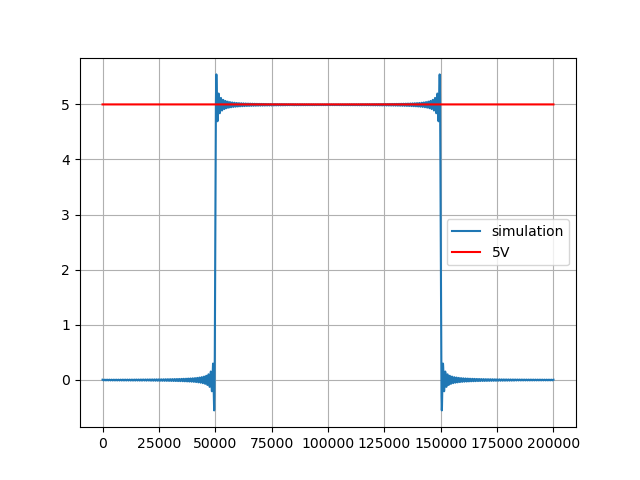
\includegraphics[width=\columnwidth]{figs/4.3.png}
			\caption{Convolution of the $x(t)$ and $h(t)$.}
			\label{eq:fig:4.3}
		\end{figure}
The following python code plots the figure \ref{fig:4.3}
\begin{lstlisting}
wget https://github.com/Pradeep8802/EE3900-Digital-Signal-Processing/blob/main/charger/codes/4.3.py
\end{lstlisting} 
\end{enumerate}
\section{Filter Design}
\begin{enumerate}[label=\thesection.\arabic*
	,ref=\thesection.\theenumi]
	\item Design a Butterworth filter for $H(f)$.\\
	\solution The Butterworth filter has an amplitude response
	given by
	\begin{align}
		\abs{H\brak{f}}^2 = \frac{1}{\brak{1 + \brak{\frac{f}{f_c}}^{2n}}}
	\end{align}
	where $n$ is the order of the filter and $f_c$ is the cutoff
	frequency. The attenuation at frequency $f$ is given by 
	\begin{align}
		A &= -10\log_{10}\abs{H\brak{f}}^2 \\
		&= -20\log_{10}\abs{H\brak{f}}
		\label{eq:loss}
	\end{align}
	We consider the following design parameters for our
	lowpass analog Butterworth filter:
	\begin{enumerate}
		\item Passband edge, $f_p = 50$ Hz
		\item Stopband edge, $f_s = 100$ Hz
		\item Passband attenuation, $A_p = -1$ dB
		\item Stopband attenuation, $A_s = -20$ dB
	\end{enumerate}
	We are required to find a desriable order $n$ and cutoff
	frequency $f_c$ for the filter. From \eqref{eq:loss},
	\begin{align}
		A_p &= -10\log_{10}\sbrak{1 + \brak{\frac{f_p}{f_c}}^{2n}} \\
		A_s &= -10\log_{10}\sbrak{1 + \brak{\frac{f_s}{f_c}}^{2n}}
	\end{align}
	Thus,
	\begin{align}
		\brak{\frac{f_p}{f_c}}^{2n} = 10^{-\frac{A_p}{10}} - 1 \label{eq:fc1} \\
		\brak{\frac{f_s}{f_c}}^{2n} = 10^{-\frac{A_s}{10}} - 1 \label{eq:fc2}
	\end{align}
	Therefore, on dividing the above equations and solving for $n$,
	\begin{align}
		n = \frac{\log\brak{10^{-\frac{A_s}{10}} - 1} - 
			\log\brak{10^{-\frac{A_p}{10}} - 1}}{2\brak{\log{f_s} - \log{f_p}}}
	\end{align}
	In this case, making appropriate susbstitutions gives $n = 4.29$.
	Hence, we take $n = 5$. Solving for $f_c$ in \eqref{eq:fc1} and
	\eqref{eq:fc2},
	\begin{align}
		f_{c1} = f_p\sbrak{10^{-\frac{A_p}{10}} - 1}^{-\frac{1}{2n}} = \SI[parse-numbers=false]{57.23}{\hertz} \\
		f_{c2} = f_s\sbrak{10^{-\frac{A_s}{10}} - 1}^{-\frac{1}{2n}} = \SI[parse-numbers=false]{63.16}{\hertz}
	\end{align}
	Hence, we take $f_c = \sqrt{f_{c1}f_{c2}} = \SI[parse-numbers=false]{60}{\hertz}$ approximately.
	\item Design a Chebyshev filter for $H(f)$.bjjk,bv,kgg
	\solution The Chebyshev filter has an amplitude response
	given by
	\begin{align}
		\abs{H\brak{f}}^2 = \frac{1}{\brak{1 + \epsilon^2C_n^2\brak{\frac{f}{f_c}}}}
	\end{align}
	where 
	\begin{enumerate}
		\item $n$ is the order of the filter
		\item $\epsilon$ is the ripple
		\item $f_c$ is the cutoff frequency 
		\item $C_n = \cosh^{-1}\brak{n\cosh{x}}$ denotes 
		the n\textsuperscript{th} order Chebyshev polynomial,
		given by
		\begin{align}
			c_n(x) =
			\begin{cases}
				\cos\brak{n\cos^{-1}x} & \abs{x} \le 1 \\
				\cosh\brak{n\cosh^{-1}x} & \textrm{otherwise}
			\end{cases}
			\label{eq:chebypol}
		\end{align}
	\end{enumerate}
	We are given the following specifications:
	\begin{enumerate}
		\item Passband edge (which is equal to 
		cutoff frequency), $f_p = f_c$
		\item Stopband edge, $f_s$
		\item Attenuation at stopband edge, $A_s$
		\item Peak-to-peak ripple $\delta$ in the passband.
		It is given in dB and is related to $\epsilon$ as
		\begin{align}
			\delta = 10\log_{10}\brak{1 + \epsilon^2}
			\label{eq:delta-eps}
		\end{align}
	\end{enumerate}
	and we must find a suitable $n$ and $\epsilon$. From
	\eqref{eq:delta-eps},
	\begin{align}
		\epsilon = \sqrt{10^{\frac{\delta}{10}} - 1}
		\label{eq:epsilon-del}
	\end{align}
	At $f_s > f_p = f_c$, using \eqref{eq:chebypol}, $A_s$ is given by
	\begin{align}
		A_s = -10\log_{10}\sbrak{1 + \epsilon^2c_n^2\brak{\frac{f_s}{f_p}}} \\
		\implies c_n\brak{\frac{f_s}{f_p}} = \frac{\sqrt{10^{-\frac{A_s}{10}} - 1}}{\epsilon} \\
		\implies n = \frac{\cosh^{-1}\brak{\frac{\sqrt{10^{-\frac{A_s}{10}} - 1}}{\epsilon}}}
		{\cosh^{-1}\brak{\frac{f_s}{f_p}}}
	\end{align}
	We consider the following specifications:
	\begin{enumerate}
		\item Passband edge/cutoff frequency, $f_p = f_c = \SI[parse-numbers=false]{60}{\hertz}$.
		\item Stopband edge, $f_s = \SI[parse-numbers=false]{100}{\hertz}$.
		\item Passband ripple, $\delta = \SI[parse-numbers=false]{0.5}{\dB}$
		\item Stopband attenuation, $A_s = \SI[parse-numbers=false]{-20}{\dB}$
	\end{enumerate}
	$\epsilon = 0.35$ and $n = 3.68$. Hence, we take $n = 4$
	as the order of the Chebyshev filter.
	\item Design a circuit for your Butterworth filter.
	\solution Looking at the table of normalized element values
	$L_k$, $C_k$, of the Butterworth filter for order 5, and noting
	that de-normalized values $L_k'$ and $C_k'$ are given by
	\begin{align}
		C_k' = \frac{C_k}{\omega_c} \qquad L_k' = \frac{L_k}{\omega_c}
	\end{align}
	De-normalizing these values, taking $f_c = 60$ Hz,
	\begin{align}
		C_1' = C_5' = \SI{1.64}{\milli\farad} \\
		L_2' = L_4' = \SI{4.29}{\milli\henry} \\
		C_3' = \SI{5.31}{\milli\farad}
	\end{align}
	The L-C network is shown in Fig. \ref{fig:butter-filter}.
	\begin{figure}[!ht]
		\centering
		\begin{circuitikz} 
			\draw (0,0) to[short, o-o] (7,0);
			\draw (0,2) to [short, o-] (1,2) to [L, l=4.29 mH] (3.5,2) to [L, l=4.29 mH] (6,2) to[short, -o] (7,2);
			\draw (1,0) to[C, l=1.64 mF] (1,2);
			\draw (3.5,0) to[C, l=5.31 mF] (3.5,2);
			\draw (6,0) to[C, l=1.64 mF] (6,2);
		\end{circuitikz}
		\caption{L-C Butterworth Filter}
		\label{fig:butter-filter}
	\end{figure}
	
	\begin{figure}
		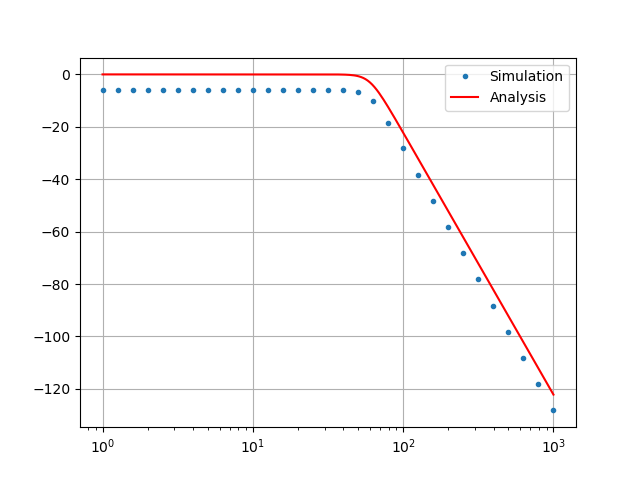
\includegraphics[width=\columnwidth]{figs/5.3.png}
		\caption{Simulation of Chebyshev filter.}
		\label{fig:sim-butter}
	\end{figure}
	Below python code plot the figure \ref{fig:sim-butter}
	\begin{lstlisting}
wget https://github.com/Pradeep8802/EE3900-Digital-Signal-Processing/blob/main/charger/codes/5.3.py
	\end{lstlisting} 

	\item Design a circuit for your Chebyshev filter.
	
	\solution Looking at the table of normalized element values
	of the Chebyshev filter for order 3 and 0.5 dB ripple,
	and de-nomrmalizing those values, taking $f_c = \SI[parse-numbers=false]{50}{\hertz}$,
	\begin{align}
		C_1' = \SI{4.43}{\milli\farad} \\
		L_2' = \SI{3.16}{\milli\henry} \\
		C_3' = \SI{6.28}{\milli\farad} \\
		L_4' = \SI{2.23}{\milli\henry}
	\end{align}
	The L-C network is shown in Fig. \ref{fig:cheby-filter}.
	\begin{figure}[!ht]
		\centering
		\begin{circuitikz} 
			\draw (0,0) to[short, o-o] (7,0); 
			\draw (1,0) to[C, l=4.43 mF] (1,2);
			\draw (3.5,0) to[C, l=6.28 mF] (3.5,2);
			\draw (0,2) to [short, o-] (1,2) to [L, l=3.16 mH] (3.5,2) to[L, l=2.23 mH] (6,2) to[short, -o] (7,2);
		\end{circuitikz}
		\caption{L-C Chebyshev Filter}
		\label{fig:cheby-filter}
	\end{figure}
	\begin{figure}
	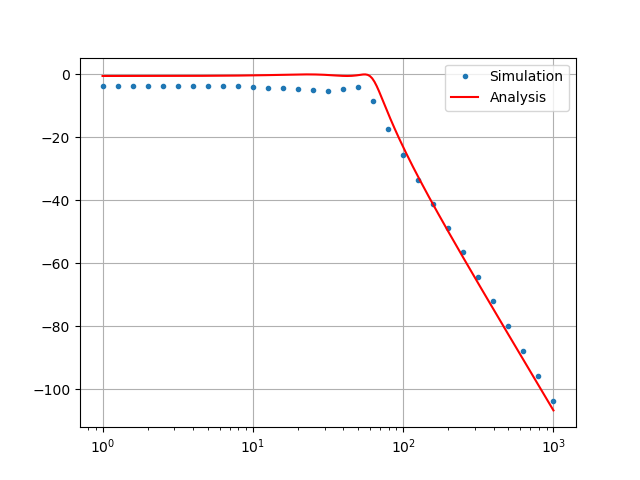
\includegraphics[width=\columnwidth]{figs/5.4.png}
	\caption{Simulation of Chebyshev filter.}
	\label{fig:sim-cheby}
\end{figure}
	Below python code plot the figure \ref{fig:sim-cheby}
	\begin{lstlisting}
wget /codes/5.4.py
	\end{lstlisting} 
\end{enumerate}


    \end{document}